\let\negmedspace\undefined
\let\negthickspace\undefined
\documentclass[journal]{IEEEtran}
\usepackage[a5paper, margin=10mm, onecolumn]{geometry}
%\usepackage{lmodern} % Ensure lmodern is loaded for pdflatex
\usepackage{tfrupee} % Include tfrupee package

\setlength{\headheight}{1cm} % Set the height of the header box
\setlength{\headsep}{0mm}     % Set the distance between the header box and the top of the text

\usepackage{gvv-book}
\usepackage{gvv}
\usepackage{cite}
\usepackage{amsmath,amssymb,amsfonts,amsthm}
\usepackage{algorithmic}
\usepackage{graphicx}
\usepackage{textcomp}
\usepackage{xcolor}
\usepackage{txfonts}
\usepackage{listings}
\usepackage{enumitem}
\usepackage{mathtools}
\usepackage{gensymb}
\usepackage{comment}
\usepackage[breaklinks=true]{hyperref}
\usepackage{tkz-euclide} 
\usepackage{listings}
% \usepackage{gvv}                                        
\def\inputGnumericTable{}                                 
\usepackage[latin1]{inputenc}                                
\usepackage{color}                                            
\usepackage{array}                                            
\usepackage{longtable}                                       
\usepackage{calc}                                             
\usepackage{multirow}                                         
\usepackage{hhline}                                           
\usepackage{ifthen}                                           
\usepackage{lscape}
\begin{document}

\bibliographystyle{IEEEtran}
\vspace{3cm}

\title{10.7.4}
\author{EE25BTECH11060 - V.Namaswi}
% \maketitle
% \newpage
% \bigskip
{\let\newpage\relax\maketitle}
\renewcommand{\thefigure}{\theenumi}
\renewcommand{\thetable}{\theenumi}
\setlength{\intextsep}{10pt} % Space between text and floats
\textbf{Question}\\
Prove that $y=2x+2\sqrt{3}$  is commom tangent to the parabola $y^2=16\sqrt{3}x$ and the ellipse $2x^2+y^2=4$\\
\textbf{Solution}\\
General Formulae of a conic\\
\begin{align}
\vec{x}^T V \vec{x} + 2 \vec{u}^T \vec{x} + f = 0
\end{align}
The tangent condition for line $\vec{n}^T \vec{x} + c = 0$ at contact point $\vec{q}$ is
\begin{align}
V\vec{q} + \vec{u} = \lambda \vec{n}\\ 
\vec{u}^T \vec{q} + f = \lambda c
\end{align}
for some scalar $\lambda$.
For Parabola $y^2 = 16\sqrt{3}\,x$
 \begin{align}
V = \begin{pmatrix}0 & 0 \\ 0 & 1\end{pmatrix}\\
\quad 
\vec{u} = \begin{pmatrix}-8\sqrt{3} \\ 0\end{pmatrix}\\
\quad 
f = 0.
\end{align}

Line: $2x - y + 2\sqrt{3} = 0$, so
\begin{align}
\vec{n} = \begin{pmatrix}2 \\ -1\end{pmatrix} \\
\quad c = 2\sqrt{3}
\end{align}

\noindent First condition
\begin{align}
V\vec{q} + \vec{u} = \begin{pmatrix}-8\sqrt{3} \\ y\end{pmatrix} 
= \lambda \begin{pmatrix}2 \\ -1\end{pmatrix}.
\end{align}
Thus $\lambda = -4\sqrt{3}$  and $y = 4\sqrt{3}$.

\noindent Second condition:
\begin{align}
\vec{u}^T \vec{q} + f = -8\sqrt{3}\,x = \lambda c = (-4\sqrt{3})(2\sqrt{3}) = -24,
\end{align}
giving $x = \sqrt{3}$.

\begin{align}
{\vec{q} = \begin{pmatrix}\sqrt{3} \\ 4\sqrt{3}\end{pmatrix}}
\end{align}

So the line touches the parabola at $(\sqrt{3}, 4\sqrt{3})$.

For Circle $2x^2 + y^2 = 4$
\begin{align}
V = \begin{pmatrix}2 & 0 \\ 0 & 1\end{pmatrix}\\
\quad 
\vec{u} = \begin{pmatrix}0 \\ 0\end{pmatrix}\\
\quad 
f = -4.
\end{align}

\noindent First condition:
\begin{align}
V\vec{q} = \lambda \vec{n}
\end{align}
we get 
\begin{align}
\vec{q} = \lambda \begin{pmatrix}1 \\ -1\end{pmatrix}.
\end{align}

\noindent Second condition:
\begin{align}
\vec{u}^T\vec{q} + f = -4 = \lambda c = \lambda(2\sqrt{3})
\quad \\ \Rightarrow \quad \lambda = -\frac{2}{\sqrt{3}}.
\end{align}

So
\begin{align}
\vec{q} = -\frac{2}{\sqrt{3}} \begin{pmatrix}1 \\ -1\end{pmatrix}
= \begin{pmatrix}-\tfrac{2\sqrt{3}}{3} \\ \tfrac{2\sqrt{3}}{3}\end{pmatrix}.
\end{align}
\begin{align}
{\vec{q} = \begin{pmatrix}-\tfrac{2\sqrt{3}}{3} \\ \tfrac{2\sqrt{3}}{3}\end{pmatrix}}
\end{align}
So the line touches the circle at $\left(-\tfrac{2\sqrt{3}}{3}, \tfrac{2\sqrt{3}}{3}\right)$.
Hence given line is common tangent to both the curves.
\begin{align}
\centering
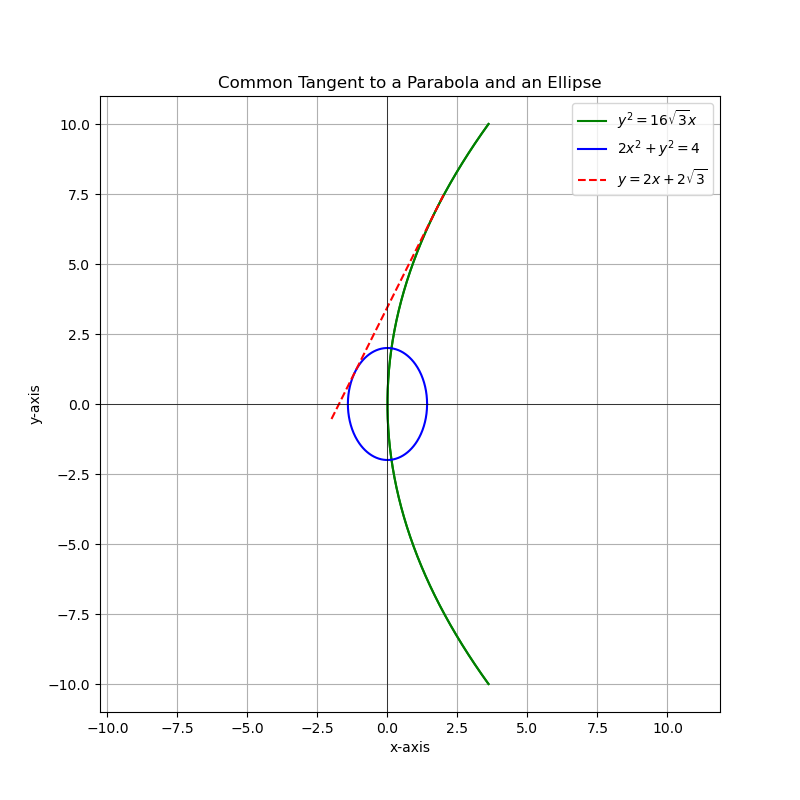
\includegraphics[width=\columnwidth, height=0.8\textheight, keepaspectratio]{figs/Figure_17.png} 
\end{align}
\end{document}
